%************************************************
\chapter{Experiment 2A: Job's Method of Continuous Variation (UV-Vis)}
%************************************************
\begin{flushright}
August 30, 2012
\end{flushright}

\section{Objective}
	To find the reaction stoichiometry of the $Fe^{3+}-$Salicylic complex using Job's method of continuous variation.

\section{Theory}
	The idea is fairly simple. We analyse a compound which is formed by a combination of two reactant substances. The only requirement is that we should know of some way using which we can quantify the compound, given a mixture consisting of the compound along with the residual reactant substances.
	\par
	Here's what we do...:
	\begin{enumerate}
		\item Decide on a total number of moles you will initially take (of both the reactant substances combined)
		\item Now take the reactant substances in various ratios, such that the total number of moles is as decided
		\item For each ratio, find out the quantity of the compound obtained
	\end{enumerate} 
	...and why:
	\par
	A little thought will make the entire procedure appear elegantly simple. In the various combinations, one of the reactants will always be a limiting reagent. However, the highest yield will be obtained in the case when the reactants are closest to the stoichiometric ratio of the compound. Thus, a plot of the concentration of the compound against that of one of the reactants will attain a maxima. The point at which the maxima is obtained, can be used to find the concentration of both reactants, whose ratio gives us the reaction stoichiometry, with respect to the reactants!
	\par
	And just to state the obvious, as the title suggests, the technique we use for quantifying is UV Visible spectroscopy.
\section{Procedure}
	As always, when practically performing an experiment, we have a few extra details to take care of.
	\begin{enumerate}
		\item Make a $0.001M$, $25mL$ solution of Iron Nitrate, $Fe(NO_{3})_{3}$.
			\begin{enumerate}
				\item The Molar Mass was given to be $404g$.
				\item Thus, for $25mL$ we need $10.0mg$.
			\end{enumerate}
		\item Make a $0.001M$, $25mL$ solution of Salicylic Acid
			\begin{enumerate}
				\item The Molar Mass was given to be $138.12g$
				\item Thus, for $25mL$, we need $3.5mg$.
			\end{enumerate}
		\item \marginpar {\Lisa Since the molarity of both solutions, is the same, we can use volume as a measure of number of moles.} We use $10mL$ as the total volume.
		\item We used the volumes given in \autoref{2A_conc}, of the reactants from the $0.001M$ solutions prepared, for creating $5mL$ solutions and marked the volumetric flasks with the corresponding concentrations.
			\begin{enumerate}
				\item Used an appropriate graduated pipette for measuring the volumes
				\item Used the pipette for measuring one of the reactants only, and filled the volumetric flask with the other reactant using a dropper, to $5mL$ using the mark on the flask. This was done to avoid errors.
				\item Each of the flasks were ensured to be dry.
			\end{enumerate}
			\begin{table}
				\myfloatalign
				\begin{tabularx}{\textwidth}{Xll}
					\tableheadline{$Fe^{3+}$ Solution's Volume ($mL$)} & \tableheadline{Salicylic Acid's Volume ($mL$)}\\
					% \tableheadline{Volume ($mL$)} & \tableheadline{Salicylic Acid Volume ($mL$)}\\
					\hline%
					$0.5$				& 	$4.5$\\
					$2.0$				& 	$3.0$\\
					$2.5$				& 	$2.5$\\
					$3.0$				& 	$2.0$\\
					$4.5$				& 	$0.5$\\
					\hline%
				\end{tabularx}
				\caption{Concentrations for Job's Method}
				\label{2A_conc}
			\end{table}
		\item Recorded the spectrum of one of the samples and found the peak corresponding to the compound we're interested in, viz. $Fe^{3+}-$Salicylate Complex.
		\item Recorded the absorbance of the frequency determined in the previous step for all concentrations.
	\end{enumerate}

\section{Observations and Analysis}
	\begin{enumerate}
		\item Characteristic wavelength was found to be $518.00$.
		\item Intensities for varying concentrations of $Fe^{3+}$ have been listed in \autoref{2A_conc_v}.
		\item From \autoref{2A_graph}, it's clear that the maximum concentration is obtained for the \emph{stoichiometric ratio of 1:1}, as the maxima is obtained very close to $2.5 mL$, which represents equal concentrations of both reactants. \marginpar{\Bart How do you know the graph will be linear on both sides? \Lisa [Product] $\alpha$ [Limiting Reactant]}
	\end{enumerate}

	\begin{table}
		\myfloatalign
		\begin{tabularx}{\textwidth}{Xll}
			\tableheadline{$Fe^{3+}$ Solution's Volume ($mL$)} & \tableheadline{Absorbance}\\
			% \tableheadline{Volume ($mL$)} & \tableheadline{Salicylic Acid Volume ($mL$)}\\
			\hline%
			$0.5$				& 	$0.350$\\
			$2.0$				& 	$0.682$\\
			$2.5$				& 	$0.801$\\
			$3.0$				& 	$0.740$\\
			$4.5$				& 	$0.282$\\
			\hline%
		\end{tabularx}
		\caption{Absorbance for Varying Concentrations}
		\label{2A_conc_v}
	\end{table}
	
	\begin{figure}[bth]
		\begin{center}
			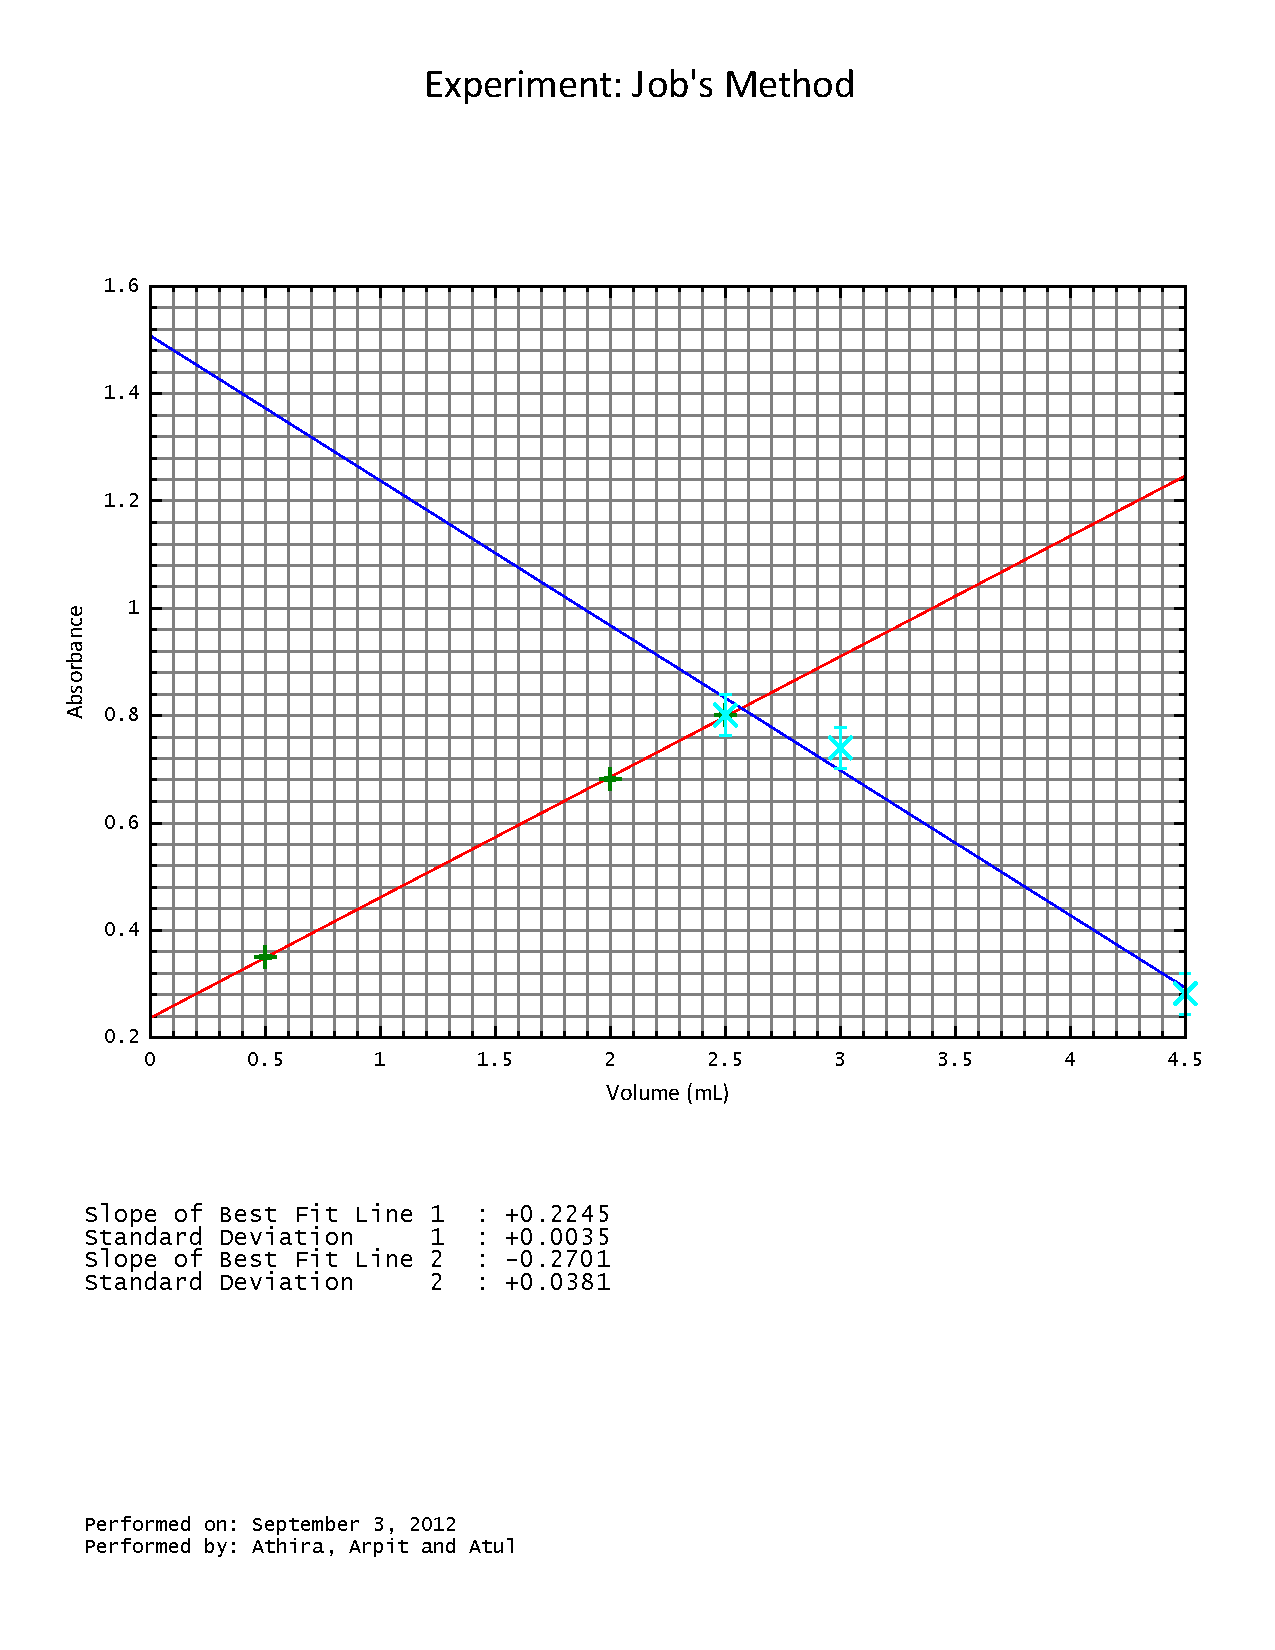
\includegraphics[width=1.2\linewidth]{gfx/2A}
		\end{center}
	\caption[Absorbance with Varying Concentrations]{\label{2A_graph}}
	\end{figure}

\section{Discussion}
	Fortunately or unfortunately, the experiment returned expected results and therefore there's no real requirement of a discussion. However, it must be mentioned that by just looking at the colour of the solution, the search can be narrowed to a great extend, that is, cases in which the product and/or reactants are coloured.\\

\section{Acknowledgements}
	I acknowledge the contribution of Mr. Arpit Porwal and Ms. Athira Nair, for the performance of the experiment as team members. I would also like to thank Ms. Ritu Roy Chowdhury for discussing the expected graph, which helped me understand the experiment better.\\